%%%%%%%%%%%%%%%%%%%%%%%%%%%%%%%%%%%%%%%%%%%%%%%%%%%%%%%%%%%%%%%
% IMPORTANTE: Cambiar el compilador a XeLaTeX en las opciones %
%     Si se quiere hacer "doble enter" usar: \vspace{2ex}     %
%               Creditos Github: @diegocostares               %
%%%%%%%%%%%%%%%%%%%%%%%%%%%%%%%%%%%%%%%%%%%%%%%%%%%%%%%%%%%%%%%
\documentclass{style}

\begin{document}
%%%%%%%%%%%%%%%%% RENOMBRE %%%%%%%%%%%%%%%%%
\graphicspath{ {./img/} }
\renewcommand{\contentsname}{Tabla de Contenido}
\renewcommand{\listfigurename}{Índice de Ilustraciones}
\renewcommand{\listtablename}{Índice de Tablas}
\renewcommand{\tablename}{Tabla}
\renewcommand{\figurename}{Figura}
\renewcommand*{\lstlistingname}{Código}

%%%%%%%%%%%% Certificado de Entrega %%%%%%%%%%%%%%%
% Se sube un pdf:
%\includepdf{content/certificado.pdf}

%%%%%% Registro de Autorización de la Práctica %%%%%%%%%
%\includepdf{content/registro.pdf}

%%%%%%%%%%%%%%%%% PORTADA %%%%%%%%%%%%%%%%%
\ThisCenterWallPaper{1}{content/Portada_practica_1.pdf}
\portada{Nombre completo} % Insertar nombre acá
        {Correo electronico} % Insertar correo acá
        {Nombre de la empresa} % Insertar empresa acá
        {\today} % Insertar fecha

%%%%% Formulario de Evaluación de la U %%%%%%%%
%\includepdf{content/formulario.pdf}

%%%%% Formulario de Evaluación de la U %%%%%%%%
%\includepdf{content/formulario.pdf}

%%%%%%%% Formulario de Evaluación de la Empresa %%%%%%%
%\includepdf{content/formulario.pdf}

%%%%%%%%%%%% Numeración paginas %%%%%%%%%%%  
\pagenumbering{arabic}
%%%%%%%%%%%%%%%%% INDICES %%%%%%%%%%%%%%%%%
\tableofcontents \newpage
\listoftables \newpage
\listoffigures \newpage
%\lstlistoflistings \newpage % Para hacer indice de codigo
%%%%%%%%%%%%%%%%% ESPACIADO %%%%%%%%%%%%%%%%%
\setstretch{1.15} 
%%%%%%%%%%%%%%%%% CONTENIDO %%%%%%%%%%%%%%%%%
\section{Tutorial: Imágenes}
\subsection{Imagen centrada}
La forma de incluir imágenes en esta plantilla es con el comando personalizado:
\begin{verbatim} 
\fig[label]{Titulo}{tamaño}{ruta_imagen}
\end{verbatim}

\fig[referencia1]{Titulo de la imagen 1}{width = 0.4\textwidth}{img/cuadradoejemplo.png}

% Tambien se puede agregar sin caption ni label ni titulo:
% \fig{}{width = 0.2\textwidth}{img/cuadradoejemplo.png}

\subsection{Imágenes alineadas}
Si se desea incluir una imagen a la izquierda o derecha de un párrafo, se puede hacer lo siguiente (Poniendo \{r\} o \{l\} dependiendo del caso):

\begin{wrapfigure}{r}{0.2\textwidth} % Margen del texto
    \centering
    \begin{measuredfigure}
        \caption{Titulo de la imagen}
        
\includegraphics[height=3cm]{img/cuadradoejemplo.png} %[scale=0.1]
        \label{img:referencia2}
    \end{measuredfigure}
\end{wrapfigure}


\textcolor{silver}{
    \lipsum[2]
}

%%%%%%%%%%%%%%%%%%%%%%%%%%%%%%%%%%%%%%%%%%%%%%%%%%%%%%%
\newpage
\section{Tutorial: Tablas}

Hacer tablas en \LaTeX es muy engorroso, por lo que presentamos 3 alternativas. Sin embargo, es necesario aclarar que para que se respete el formato de las tablas, \textbf{se tiene que poner el catión SOBRE la tabla.}

\subsection{Generador online}
Hay muchas páginas para generar tablas automáticamente, una alternativa es \href{https://www.tablesgenerator.com}{tablesgenerator}, sin embargo, este método genera muchas líneas innecesarias y cuando se incorporan párrafos muy grandes hay que ajustar las palabras.

\subsection{Insertar una imagen como tabla}
Se puede incorporar una imagen (De Excel, por ejemplo) como si fuera una tabla. El único inconveniente es que no va a permitir seleccionar el texto en el pdf generado.
\begin{table}[H]
    \centering
    \caption{Tabla de referencia 1}
    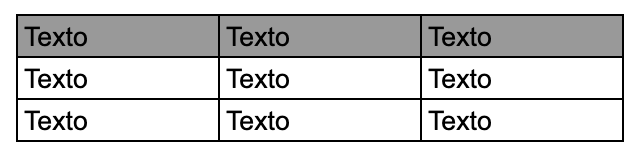
\includegraphics[height=3cm]{img/tablaejemplo.png} 
    \\ \scriptsize{Texto opcional al el pie de Tabla.}
    \label{img:referencia3}
\end{table}


\subsection{Usar plantilas}
\begin{minipage}[H]{0.49\textwidth}
    \begin{table}[H]
        \centering
        \caption{Tabla de referencia 2}
        \begin{tabular}{| l | c | r |} 
        \hline
            \textbf{Texto} & \textbf{Texto} & \textbf{Texto} \\ \hline
            Textoblabla    & Textoblabla   & Textoblabla \\ \hline
            Texto    & Texto   & Texto \\ \hline
        \end{tabular}
        \\ \scriptsize{Texto opcional al el pie de Tabla.}
    \end{table}
\end{minipage}
\begin{minipage}[H]{0.49\textwidth}
    \begin{table}[H]
        \centering
        \caption{Tabla de referencia 3}
        \begin{tabular}{l l l}
        \toprule
            \textbf{Texto} & \textbf{Texto} & \textbf{Texto} \\
            \midrule
            Textoblabla    & Textoblabla   & Textoblabla \\
            Texto    & Texto   & Texto \\
            \bottomrule
        \end{tabular}
        \\ \textit{\scriptsize{Texto opcional al el pie de Tabla.}}
    \end{table}
\end{minipage} % Eliminar archivo y linea
% -----------

%%%% Estas secciones son a modo de ejemplo %%%%

\section{INTRODUCCIÓN}

IMPORTANTE: estas secciones son a modo de ejemplo, no lo tomes como que debe ser así.

\subsection{Descripción de la empresa}

\subsection{Rol del estudiante}

\subsection{Objetivos del proyecto}



\subsection{Competencias de egreso}

\newpage
\section{TRABAJO REALIZADO POR EL ESTUDIANTE}
\subsection{Metodología de trabajo} 
\subsection{Desarrollo técnico del proyecto}



\subsection{Resultados obtenidos}


\newpage
\section{COMPETENCIAS DEMOSTRADAS}

\newpage
\section{CONCLUSIONES}
 % <----- ACA SE ESCRIBE

%%%%%%%%%%%%%%%%% BIBLIOGRAFIA %%%%%%%%%%%%%%%%%
\newpage
% Hay 2 formas de agregar bibliografia:
% 1. Agregar una bibliografia en un archivo .bib (Es super automatico)
% \bibliographystyle{apacite}
% \bibliography{mybib.bib} % Requiere crear un archivo .bib

% 2. Agregar una bibliografia en un archivo .tex 
% (Es manual, pero comodo para los que no conoce el bibtex)
\indent
\section{REFERENCIAS BIBLIOGRÁFICAS}
\leftskip 0.3in
\parindent -0.3in

%%%%%%%%%%%%%%% ESCRIBIR DEBAJO EN FORMATO APA %%%%%%%%%%%%%%%
% las lineas de arriba permiten que tenga una sangría francesa.


%%%%%%%%%%%%%%%%% ANEXOS %%%%%%%%%%%%%%%%%
%
\begin{center}
\vspace*{\fill}
    
\textbf{ANEXOS}
\addcontentsline{toc}{section}{ANEXOS}
\vspace*{\fill}
\end{center}
\newpage



%%%% para agregar sectiones o subsecciones al anexo ocupar 
%%%% \addannexsec{--title name--}
%%%% \addannexsubsec{--title name--}
\startannex{A}{Panel de reportería de finanzas}



\end{document}